\documentclass[addpoints,11pt]{exam}
\usepackage[top=0.5in, bottom=0.5in, left=0.5in, right=0.5in]{geometry}
\usepackage[utf8]{inputenc}
\usepackage{listings}
\usepackage{color,graphicx}
\usepackage{multicol}
\usepackage{MnSymbol}

%Impostazioni box punti - package exam
\boxedpoints
\pointname{~punti}

%Impostazioni box soluzioni - package exam
\newcommand{\makenonemptybox}[2]{%
	\par\nobreak\vspace{\ht\strutbox}\noindent
	\fbox{%
		\parbox[c][\dimexpr#1-2\fboxsep][t]{\dimexpr\linewidth-2\fboxsep}{
			\hrule width \hsize height 0pt
			#2
		}%
	}%
	\par\vspace{\ht\strutbox}
}


%Impostazioni grafiche per visione codice sorgente - linguaggio C
\definecolor{codegray}{rgb}{0,0,0}
\definecolor{backcolour}{rgb}{1,1,1}

\lstdefinestyle{mystyle}{
	backgroundcolor=\color{backcolour},   
	keywordstyle=\color{black},
	numberstyle=\tiny\color{codegray},
	basicstyle=\footnotesize,
	breakatwhitespace=false,         
	breaklines=true,                 
	captionpos=b,                    
	keepspaces=true,                 
	numbers=left,                    
	numbersep=5pt,                  
	showspaces=false,                
	showstringspaces=false,
	showtabs=false,                  
	tabsize=2
}

\lstset{style=mystyle}

\pagestyle{empty}


%Creazione documento
\begin{document}
    
%------------------------- INTESTAZIONE COMPITO -----------------------------------
\begin{center}
	\fbox{\fbox{\parbox{7in}{\centering
				Prova scritta Programmazione Procedurale con Lab. - Cerami Cristian}}}
\end{center}

\vspace{5mm}

\noindent\makebox[\textwidth]{Nome e Cognome: \rule{8cm}{.1pt} \hspace{1cm} Matricola:  \rule{5cm}{.1pt}}

\begin{questions}

%------------------------- ESERCIZIO 1 --------------------------------------------

\question[5]
Cosa stampa il seguente frammento di codice?

\begin{minipage}[t]{0.4\linewidth}
	\begin{lstlisting}[language=C]
	int a = 0123 ^ 0x056;
	double b = 2.59;

	printf ("%d\n", a);
	
	while ((++a || a++) ? a-=1 : 0) {
		if (!(a-- && --a ))
			break;
		else {
			printf("%d\n", a); 
		}
	}
	
	a<=a, a+=b, a++;
	printf("a: %d\n", a); 
	\end{lstlisting}
\end{minipage}
\begin{minipage}[t]{0.6\linewidth}
	\makenonemptybox{120pt}{~\\
	5\\
	3\\
	1\\
	-1\\
	a: 4}
\end{minipage}

%------------------------- FINE ESERCIZIO 1 ---------------------------------------

%------------------------- ESERCIZIO 2 --------------------------------------------

\question[6]
Elencare le conversioni di tipo \underline{implicite} (\emph{... da ... a}). Scrivere cosa viene stampato a schermo sapendo che: \emph{UCHAR\_MAX = 255} , \emph{'a' = 97} .

\begin{minipage}[t]{0.4\linewidth}
	\begin{lstlisting}[language=C]
	double fun (float a) {
		char b = ('x' * 3) - 'g';
		return (a / b);
	}
	
	int main (void) {
		unsigned int a = 'g' - 3UL;
		float b = fun(a);
		unsigned char c = -(int) (b+53);
		printf("c: %c, %d\n", c, c);
		return 0;
	}
	\end{lstlisting}
\end{minipage}
\begin{minipage}[t]{0.6\linewidth}
	\makenonemptybox{200pt}{~\\
linea 7: 'g' convertito da int a unsigned long int\\
linea 7: il valore dopo l'uguale è convertito da unsigned long int ad unsigned int\\
linea 8: parametro "a" di fun convertito da unsigned int a float\\
linea 2: il valore dopo l'uguale è convertito da int a char\\
linea 3: "b" è convertito da char a float per la divisione\\
linea 3: il risultato della divisione è convertito da float a double\\
linea 8: il valore di ritorno è convertito da double a float\\
linea 9: 53 è convertito da int a float\\
linea 9: il valore dopo l'uguale è convertito da int (dopo la conversione esplicita) a unsigned char\\

A schermo viene stampato ``c: g, 103'' perchè: \\c = (UCHAR\_MAX + 1) - 153 = 103 = 'g' in ASCII\\
}
\end{minipage}

%------------------------- FINE ESERCIZIO 2 ---------------------------------------

%------------------------- ESERCIZIO 3 --------------------------------------------

\question[6]
Data la seguente \emph{struct}, scrivere la definizione di una funzione di nome \emph{ritorna\_dispari} che prende come parametro una lista (\emph{lista\_input}) e ritorna un'altra lista (\emph{lista\_output}, creata nella funzione) che contiene, nello stesso ordine della lista passata, solamente gli elementi in posizione \emph{dispari} (se presenti). Se la lista originale è \textbf{5-2-9}, la lista ritornata sarà \textbf{5-9}.

\begin{minipage}[t]{0.4\linewidth}
	\begin{lstlisting}[language=C]
	typedef struct node Node;

	struct node {
		int info;
		struct node* pNext;
	};
	\end{lstlisting}
\end{minipage}
\begin{minipage}[t]{0.6\linewidth}
	\makenonemptybox{30pt}{
		\centering 
		\vspace{0.8em} 
		Guarda soluzione in fondo al compito
	}
\end{minipage}

%------------------------- FINE ESERCIZIO 3 ---------------------------------------

\newpage

%------------------------- INTESTAZIONE COMPITO -----------------------------------
\begin{center}
	\fbox{\fbox{\parbox{7in}{\centering
				Prova scritta Programmazione Procedurale con Lab. - Cerami Cristian}}}
\end{center}

\vspace{5mm}

\noindent\makebox[\textwidth]{Nome e Cognome: \rule{8cm}{.1pt} \hspace{1cm} Matricola:  \rule{5cm}{.1pt}}


%------------------------- ESERCIZIO 4 --------------------------------------------

\question[7]
Dire quali compilazioni provocano errore a causa del linker (e perchè):\\
1) gcc -o write write.c\\
2) gcc -c main.c\\
3) gcc -o main main.c\\
4) gcc -o execute main.c write.c\\
In caso il punto 4) ritorni un errore, descrivere come può essere corretto. Infine, \textbf{dopo la correzione} eventualmente applicata, elencare tutte le definizioni, dichiarazioni e tipologie di linkage, presenti in ogni file, per \emph{count}, \emph{i}, \emph{a}, e \emph{mywrite}. Cosa stampa il programma?

\begin{minipage}[h]{0.5\linewidth}
	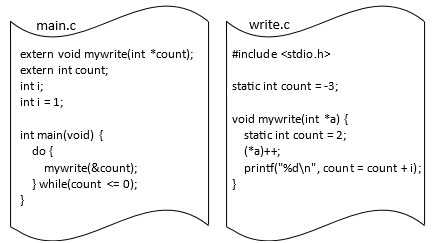
\includegraphics[width=9cm, keepaspectratio]{immagini/es_linkage_uniti}
	\begin{minipage}[h]{0.95\linewidth}
		\makenonemptybox{240pt}{
			~\\
			Stampa:\\
			3\\
			4\\
			5\\
			6\\
		}
	\end{minipage}
\end{minipage}
\begin{minipage}[h]{0.5\linewidth}
	\makenonemptybox{385pt}{
1) Manca definizione \emph{main} ed \emph{i}\\
3) Manca definizione \emph{mywrite} e \emph{count}\\
4) Manca definizione \emph{count} in \emph{main.c} perchè \emph{count} ha linkage interno in \emph{write.c} quindi non è visibile. Manca poi la dichiarazione con linkage esterno di \emph{i} in \emph{write.c}\\

Il punto 4) può essere corretto cambiando la tipologia del linkage di \emph{count} (globale) in \emph{write.c} da interno a esterno. Si fa eliminando la keyword ``\emph{static}'': \\\texttt{int count = -3;}\\
Va inoltre inserita in \emph{write.c} la dichiarazione di \emph{i} con linkage esterno: \texttt{extern int i;} \\

In main.c:\\
- \emph{mywrite} è dichiarata ed ha linkage esterno\\
- \emph{count} è dichiarata ed ha linkage esterno\\
- \emph{i} a riga 3 è un tentativo di definizione e ha linkage esterno\\
- \emph{i} a riga 4 è ora definita e ha linkage esterno\\

In write.c:\\
- DOPO LA CORREZIONE: \emph{count} a riga 3 è definita e ha linkage esterno\\
- \emph{i} è dichiarata ed ha linkage esterno\\
- \emph{mywrite} è definita e ha linkage esterno\\
- \emph{a} locale in mywrite è definita e ha no linkage\\
- \emph{count} locale in mywrite è definita e ha no linkage\\
}
\end{minipage}


%------------------------- FINE ESERCIZIO 4 ---------------------------------------

%------------------------- ESERCIZIO 5 --------------------------------------------

\question[6]
Cerchiare le affermazioni vere dato:\\ 
\underline{\emph{int a[7]= \{21,-21,[3]=INT\_MAX, 65537, [6]=511\}; short *ptr = (short*) a; char *n = (char*) a;}} ~~sapendo che i tre tipi usati occupano 4, 2 e 1 byte e 65536 = $2^{16}$ (valori rappresentati in complemento a due e \emph{little endian}). Rappresentare la zona di memoria in cui è memorizzato l'array.\\~

\textbf{A.} n+5 >= \&ptr[3]; \textbf{B.} *(n+5) > *(n+4); \textbf{C.} \&ptr[8] == ptr+9; \textbf{D.} ((int)(ptr+8)-(int)(\&a[2]) < 8);\\ \textbf{E.} *(ptr+1) == *(a+2)


\end{questions}

    %------------------------- SOLUZIONE ESERCIZIO 3 --------------------------------------------

\begin{minipage}[h]{\linewidth}
	SOLUZIONE ESERCIZIO 3
    \begin{lstlisting}[language=C]
Node* ritorna_dispari(Node* lista_input) {
	
	if (lista_input == NULL) {
		return NULL;
	} else {
		int counter = 0;
		Node* pScan = lista_input;
		
		Node* lista_output = NULL;
		Node* lista_output_pLast = NULL;
		
		while (pScan != NULL) {
			if (counter % 2 == 0) {
				Node* pNew = (Node*) malloc(sizeof(Node));
				pNew -> info = pScan -> info;
				pNew -> pNext = NULL;
				
				if (lista_output == NULL) {
					lista_output = pNew;
					lista_output_pLast = pNew;
				} else {
					lista_output_pLast -> pNext = pNew;
					lista_output_pLast = pNew;
				}	    		
			}
			
			pScan = pScan -> pNext;
			counter++;
		}
		
		return lista_output;
	}
}
	\end{lstlisting}
\end{minipage}

\begin{minipage}[h]{\linewidth}
SOLUZIONE ESERCIZIO 5\\


10101000\hspace{2em}    a[0]\\
00000000\\    
00000000\hspace{2em}    *(ptr+1)\\
00000000\\
\\
11010111\hspace{2em}    *(n+4)\\
11111111\hspace{2em}    *(n+5)\\
11111111\hspace{2em}    \&ptr[3]\\
11111111\\
\\
00000000\hspace{2em}    *(a+2) e a[2]\\
00000000\\
00000000\\
00000000\\
\\
11111111\\
11111111\\
11111111\\
11111110\\
\\
10000000\hspace{2em}    \&ptr[8] o ptr+8\\
00000000\\
10000000\hspace{2em}    ptr+9\\
00000000\\
\\
00000000\\
00000000\\
00000000\\
00000000\\
\\
11111111\\
10000000\\
00000000\\
00000000\\
\\

A = FALSO, (n+5) sta in una cella di memoria inferiore a (\&ptr[3])\\
B = VERO, ∗(n+5) == -1, ∗(n+4) == -21 quindi -1 > -21\\
C = FALSO, ricordati che si sta guardando l'indirizzo di memoria e non il loro contenuto\\
D = FALSO, la differenza in byte tra i due puntatori è 8\\
E = VERO, *(ptr+1) == 0, *(a+2) == 0 quindi *(ptr+1) == *(a+2)\\

\end{minipage}

\end{document}
